% !TEX root=main.tex

\section{Comparison: Relative Edge vs. Pose Optimization}

% show that they are equivalent
It can be plainly observed from comparing Eq~\ref{eqn:global_opt} and Eq~\ref{eqn:relative_opt} that relative edge optimization simply parametertizes the same cost function with relative edge constraints as opposed to global constraints, and therefore should result in an equivalent solution.  However, due to the different linearization between the two parameterizations, a simulation study was performed to show the equivalence of global pose and edge-based optimization. This was performed by optimization of a house-shaped trajectory, shown in Figure~\ref{fig:house_trajectory} which was corrupted with random gaussian noise, had a random selction of edges were reversed and a loop closure placed between nodes at the bottom left corner of the trajectory. This was repeated 10,000 times.  To evaluate performance of these optimizations, we employed the following RMS error metric, which can be described as the difference between the optimized global pose positions found by optimizer $j$ and optimizer $l$.

\begin{align}
    J_{RMS}(\xhat^j, \xhat^l) = \sum_{i=0}^n \lVert \xhat^j_i - \xhat^l_i \rVert
\end{align}

In the case of low heading error, every one of these optimizations produced virtually identical results between global pose and edge-based optimization.  A histogram of RMS error between the global pose of each node of the solution found by both optimizations is shown in Figure~\ref{fig:convergence_house}.  The iSAM2 package implemented in GTSAM was used as the global pose optimization algorithm, while an implementation of Algorithm~\ref{algo:reversed} was used for relative edge optimization.  It should be noted that the addition of small translation noise in the trajectory results in a global minima of the optimization problem not located at the true trajectory.  This is typical of all pose graph optimizations as described by~\cite{POSE_GRAPH_ERROR}.  Therefore, the optimization approaches are best compared directly with one another, rather than against the ground truth.

\begin{figure}
  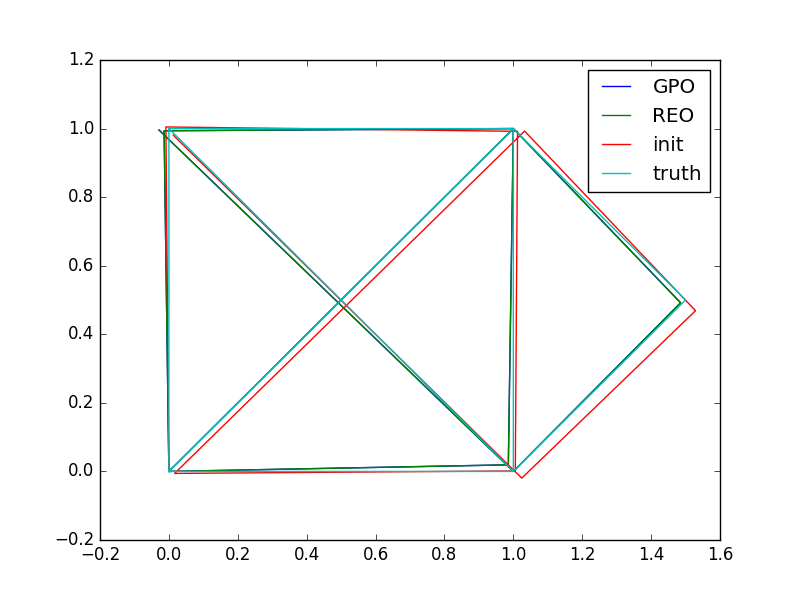
\includegraphics[width=0.7\textwidth]{figures/house_trajectory.png}
  \caption{One sample from the house trajectory simulation study with small errors in both translation and heading with identical optimization results from relative edge optimization and global pose optimization}
  \label{fig:house_trajectory}
\end{figure}

\begin{figure}[H]
  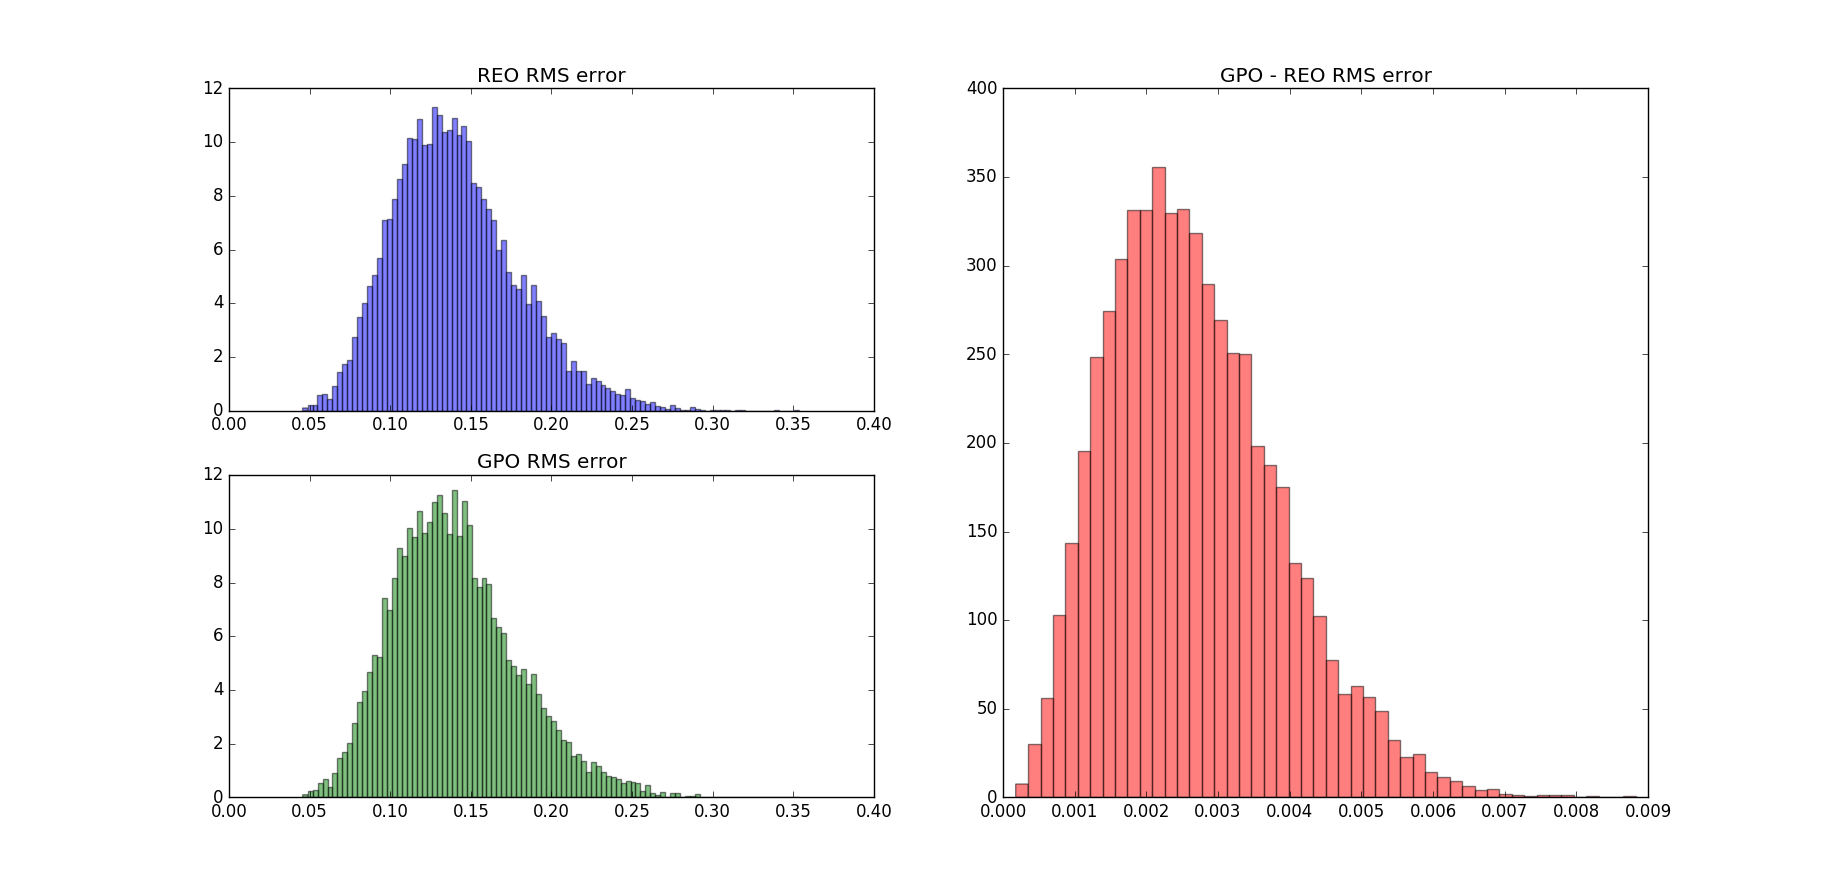
\includegraphics[width=\textwidth]{figures/REO_vs_GPO_good.png}
  \caption{RMS error between optimized poses found by relative edge optimization (REO) and global pose optimization (GPO) for a simulation study of 10,000 house trajectories with small errors in both translation and heading.}
  \label{fig:convergence_house}
\end{figure}

% describe differences (pros/cons)
% Talk about crazy heading error
Differences between the performance of global pose graph and relative edge-based optimizations can be observed by stressing linearization errors in the various parameterizations.  As a first example, a random house trajectory was generated with perfect translation measurements, but heading errors sampled from $\mathcal{N}(0, 40^\circ)$. Five perfect randomly assigned loop closures were added to the trajectory and the trajectory was given to both GPO and REO.  This process was also repeated 10,000 times.  Figure~\ref{fig:GPO_heading_divergence} shows an example of one of these trajectories, and a histogram of the RMS error of the two approaches is shown in Figure~\ref{fig:GPO_bad_histogram}. REO was able to find the true solution to within 0.001m for 90\% of the trajectories, with a max error of 0.0100m and mean of 0.0004585m.  GPO converged to within 0.001m on only a single trajectory, had a max error of 9.825$\times 10 ^{39}m$ and a mean error of 9.856$\times 10 ^{35}$.

\begin{figure}[H]
  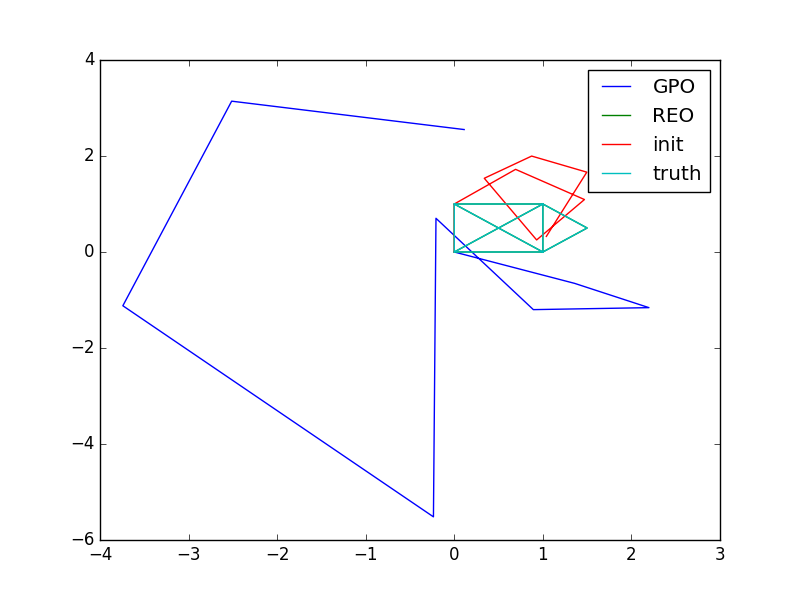
\includegraphics[width=0.7\textwidth]{figures/GPO_diverged.png}
  \caption{One sample from simulation study with perfect translation measurements, five randomly assigned perfect loop closure constraints and significant heading error.  In this case, REO found the true solution while GPO diverged.}
  \label{fig:GPO_heading_divergence}
\end{figure}

\begin{figure}[H]
  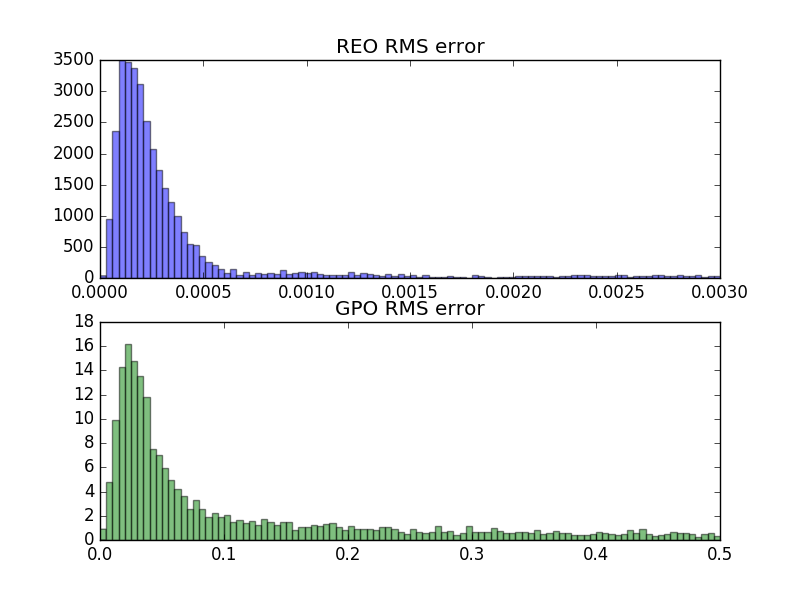
\includegraphics[width=0.7\textwidth]{figures/GPO_vs_REO_bad.png}
  \caption{histogram of RMS error calculated for the final global position of each node after each of 10,000 optimizations with significant heading error, but perfect translation measurements and five randomly assigned, perfect loop closure constraints. The maximum value of RMS error for REO in this study was 0.01004m and the maximum value of RMS error for GPO was 9.825$\times 10 ^{39}m$. Both histograms have been truncated to show details of the histogram at lower values of RMS error despite having quite long tails.}
  \label{fig:GPO_bad_histogram}.
\end{figure}

% Talk about bad initialization
Another simulation study was performed in which the house trajectory was initialized with a 180$^\circ$ heading error, and provided global measurements via a virtual zero per the method described in~\cite{CITE}. the global pose optimization often struggles to find the global minimum.  A similar experiment with 10,000 house trajectories was performed, except with the addition of a global measurement located at the peak of the house.  In this study, the pose graph optimization failed to converge to the correct optimum (As shown in Figure~\ref{fig:GPO_heading_divergence}) $20\%$ of the time, came to the same result but took more iterations as relative edge optimization $50\%$ of the time, and performed equivalently (same number of iterations, same result) the remaining $30\%$ of the time.

While relative edge optimization promises significant improvements in dealing with initialization errors when compared with global pose optimization, it is not as easily scaleable as global pose graph optimization.  In particular, the calculation of $\frac {\partial\Delta t_{a-z}}{\partial\Delta t_{ij}}$ causes significant correlations between edge estimates in a loop closure.  This ultimately leads to a loss of sparsity in the calculation of $\mathbf{H}_{az}^\top \Omega_{az} \mathbf{H}_{az}$ in Equation~\ref{eqn:3d_opt}.  The parameterization of global pose optimization however, does not run into this issue and can therefore exploit sparsity in solving for $\Delta \mathbf{x}$.  This becomes most important when considering a loop closure with a large number of edges where a dense matrix decomposition can be very costly. Secondly, in typical pose graph implementation, the number of edges can grow explosively if an agent repeatedly navigates the same area.  In this situation, the sum in the second term of the cost function in Equation~\ref{eqn:cost_function} can become extremely large and costly to calculate.

% how to use them together
To overcome these issue, we propose a two-fold solution.  To reduce the number of terms summed in the second term of Equation~\ref{eqn:cost_function}, we propose stochastically iterating over smaller loop closures in a well-connected pose graph and optimizing only a selection at a time.  To reduce the size of the optimization, we will exploit the relative nature of edge-based optimization to recursively break the full optimization into small, easy-to-manage problems.  This recursive process has the added benefit of producing completely parallelizeable independent computations which can be distributed to a GPU for fast evaluation.  While these solutions improve the scaleability of edge optimization, it still does not compete with the state-of-the-art global pose graph optimization libraries in terms of speed.  Due to the different parameterization, however, it can quickly bring a poorly initialized graph into a region where global pose graph optimization can quickly and reliably converge to a solution.  Therefore, we propose that edge optimization be performed for just a few iterations in situations where global pose graphs may struggle to find global minima to initialize the graph.  After much of the error has been removed by the more expensive, but less sensitive edge optimization, global pose graph optimization can very quickly find a global minima even in highly-connected and complicated graphs, where repeated edge optimization may become intractable.
